\documentclass[ignorenonframetext]{beamer} 

\usepackage[utf8]{inputenc} 
\usepackage{amsmath} 
\usepackage{amsfonts} 
\usepackage{amssymb} 
\usepackage[font=small]{caption} 



\mode<presentation> 
{ 
  \usetheme{Singapore} 
  \usecolortheme[named=darkgray]{structure} 

} 


\usepackage[]{algorithm2e}
\renewcommand{\figurename}{Figure}
%Standard Angaben
\author{Andrej}
\title{Foobar}
\date{\today}
\begin{document}
%---------------------------------------------1 FOLIE ---------------------------------------------
\section{}
\begin{frame}
\frametitle{

\begin{huge}
Desert ant navigational behaviour
\end{huge}

}
\ \\
\ \\
\ \\

\begin{center}

Presentation 15th of December 2015\\
\ \\
\ \\
\ \\
\begin{LARGE}
Ants in the Pants\\
\end{LARGE}
Florian Hasler, Matthias Heinzmann, Andreas Urech, Dominik Werner

\end{center}

\end{frame}












\section{Introduction}
\subsection{What is it all about?}
%---------------------------------------------2 FOLIE ---------------------------------------------














\begin{frame} 
\frametitle{What is it all about?}



\only<1>{
 \begin{figure}[H]
 \centering
 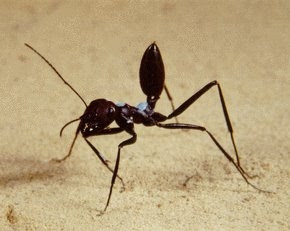
\includegraphics[scale=0.6]{./Pics/meisi.png} 
 \caption{Cataglyphis Fortis \footnote{http://www.lambrinos.ch December 5th 2015} \label{fig:Variance} }
 \end{figure}  
\begin{center} 
\end{center} 
}


\only<2>{
Some facts:
\begin{itemize}
\item one ant,  one prey $\rightarrow$ no further communication needed
\item Why is time, hence the shortest way back so crucial?
\item Distances in relation to ant's size.\\
Speed of cataglyphis fortis $\approx 1 \frac{m}{s}$
\end{itemize}
}




\only<3>{
 \begin{figure}[H]
 \centering
 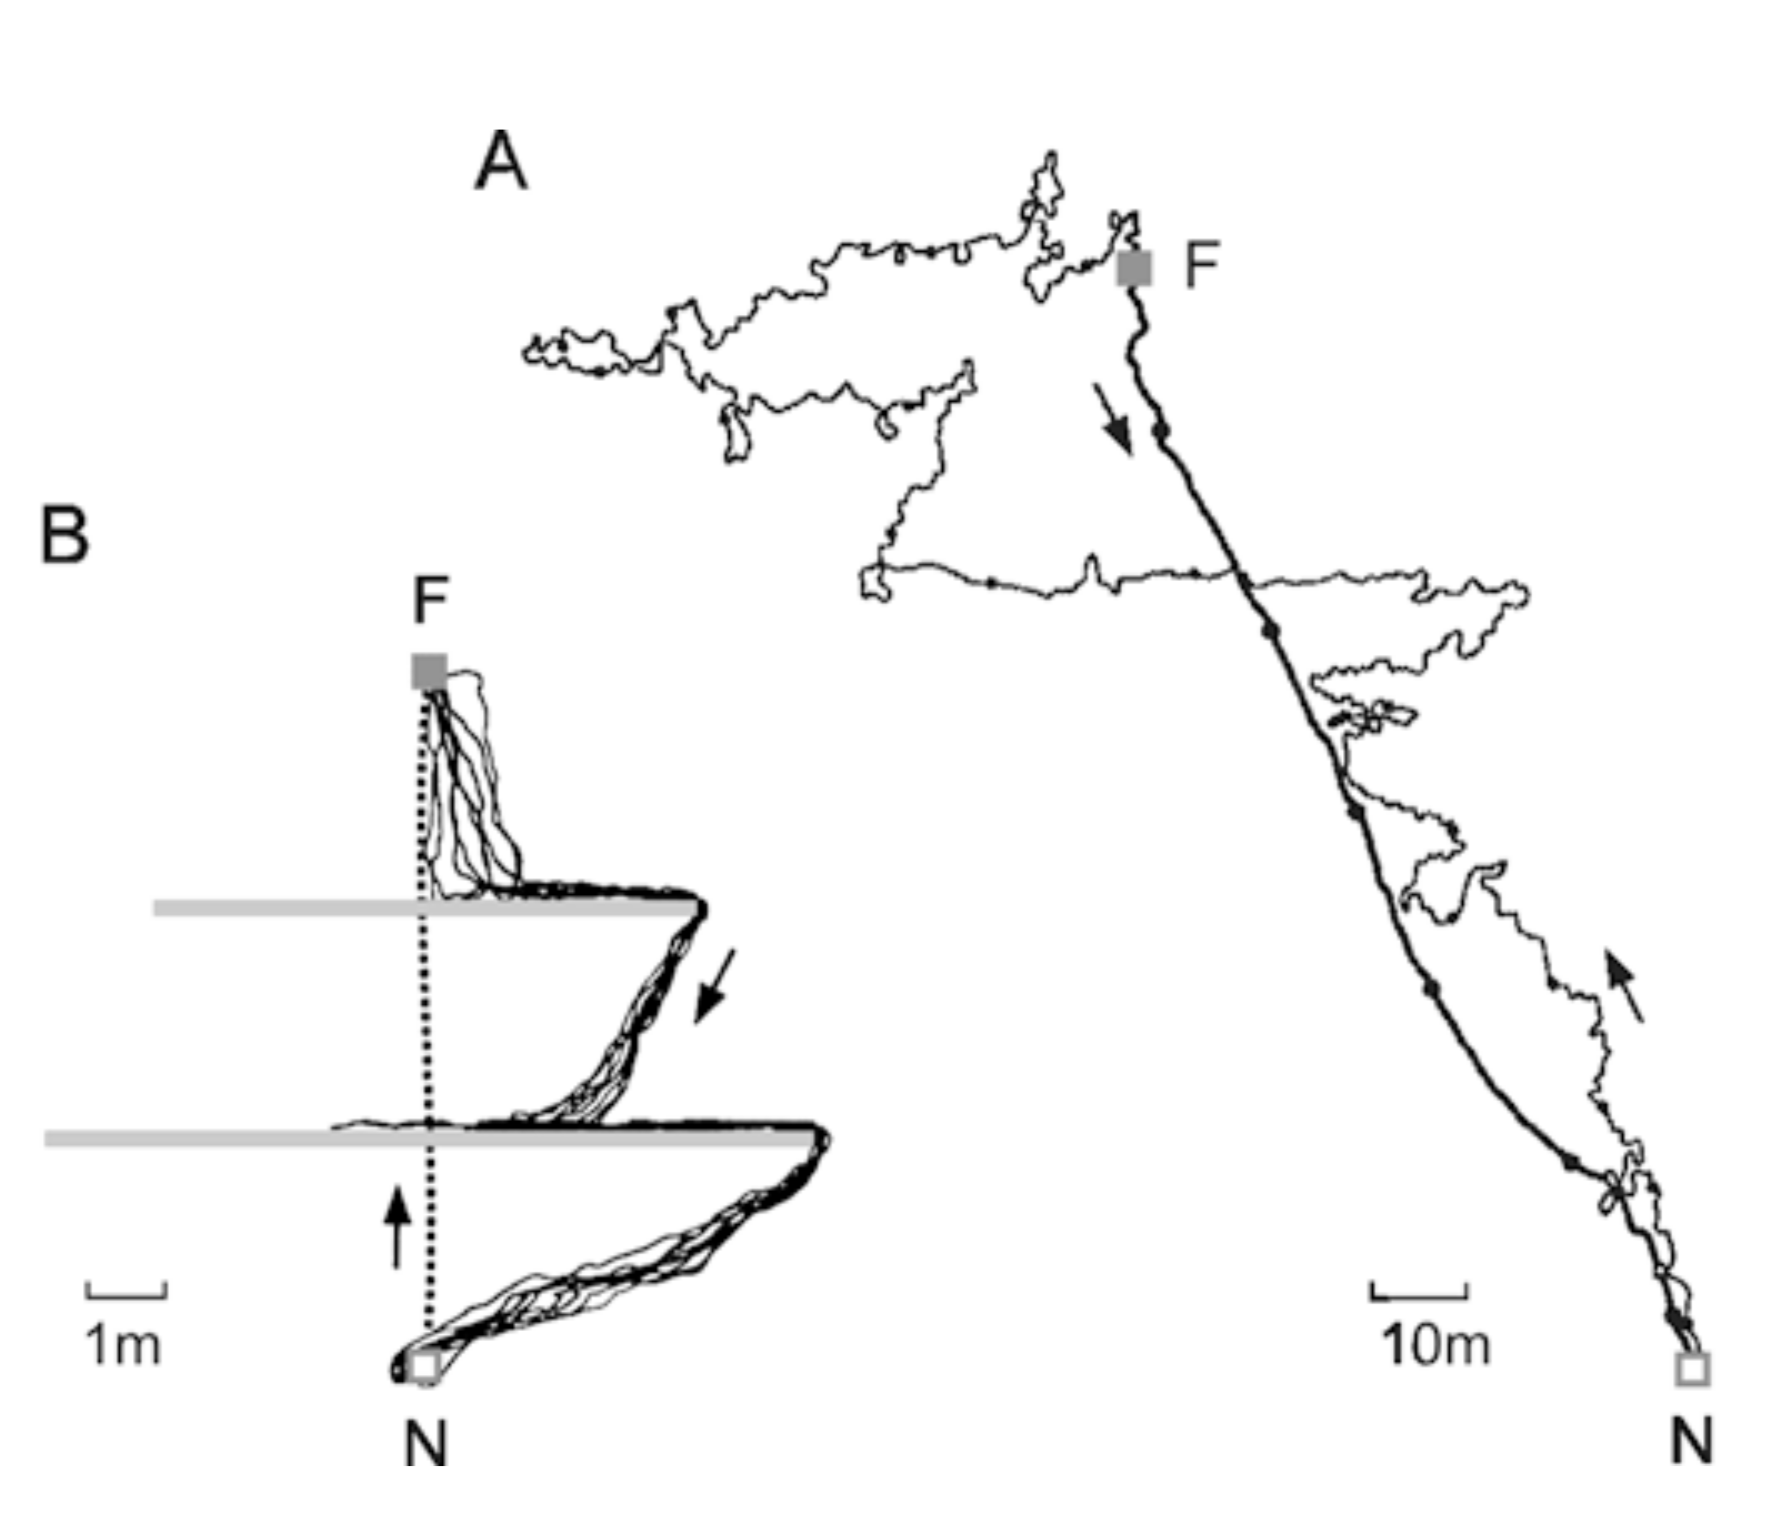
\includegraphics[scale=0.6]{./Pics/WhatAbout.png} 
 \caption{Foraging walks Wehner2003 \label{fig:Variancea} }
 \end{figure} 
\begin{center} 
\end{center} 
}




\end{frame} 













\subsection{How do they do it?}

\begin{frame} 
\frametitle{How do they do it?} 
\begin{center} 
\only<1>{ 
\begin{itemize}
\item Path integration
\end{itemize}
 } 
% 
\only<2>{ 
\begin{itemize}
\item Path integration and
\item Local Orientation
\end{itemize}
} 
%
\only<3>{ 
\begin{algorithm}[H]

  \SetKwFunction{algo}{ReturnToMyNest}
  \SetKwProg{myalg}{Algorithm}{}{}
  \myalg{\algo{}}{




%\SetKwFunction{goToMyNest}{goToMyNest}
%\goToMyNest
 \While{not at nest}{ 
 execute global vector;\\
 update global vector;
 
  \If{local vector recognised}{
   		\While{local vector $ > 0$}{
   		 execute local vector\;
   		 update local vector\;
   		 update global vector;
   			}
		}
}
 \Return
 } 
\caption{Returning to the nest}
\end{algorithm}
} 

\end{center} 
\end{frame} 
\section{Motivations Goals}
\begin{frame}
\frametitle{Motivations Goals}


\only<1>{
\begin{itemize}
\item is the path integrator model Wehner1988 applicable for general scenarios or only within the tight constraints given by the experiment of Wehner1988?
\end{itemize}
}

\only<2>{
\begin{itemize}
\item is the path integrator model Wehner1988 applicable for general scenarios or only within the tight constraints given by the experiment of Wehner1988?
\item are we able to predict what happens, when we alter the environment?
\end{itemize}
}


\only<3>{
\begin{itemize}
\item is the path integrator model Wehner1988 applicable for general scenarios or only within the tight constraints given by the experiment of Wehner1988?
\item are we able to predict what happens, when we alter the environment?
\item Can the ants survive if we rid the environment completely of any landmarks?
\end{itemize}
}



\end{frame}

\section{Path integrator}



\subsection{Pahtintegrator-model}
\begin{frame}
\frametitle{Path integrator-model \footnote{Wehner1988}}
\begin{align*}
\varphi_(n+1) =& \varphi(n) +k \cdot \frac{(\pi +\delta)\cdot(\pi-\delta)\cdot \delta}{l(n)}\\
l(n+1) =& l(n) +1 -\frac{|\delta|}{\pi}
\end{align*}
where $k = 0.1316$ is a fitting constant , $\delta$ is the angle with which the ant is turning its current direction and the step width is assumed to be 1.







\end{frame}

\subsection{Discussion of the path integrator}
\begin{frame}
\frametitle{Discussion of the path integrator}


\only<1>{
\begin{figure}[H]
\centering
\includegraphics[scale=0.5]{./Pics/0_degrees.jpg} 
\caption{0 degrees }
\end{figure} 
} 


\only<2>{
\begin{figure}[H]
\centering
\includegraphics[scale=0.5]{./Pics/40_degrees.jpg} 
\caption{40 degrees }
\end{figure} 
} 


\only<3>{
\begin{figure}[H]
\centering
\includegraphics[scale=0.5]{./Pics/80_degrees.jpg} 
\caption{80 degrees }
\end{figure} 
} 


\only<4>{
\begin{figure}[H]
\centering
\includegraphics[scale=0.5]{./Pics/120_degrees.jpg} 
\caption{120 degrees }
\end{figure} 
} 
\end{frame}



\subsection{Discussion of the ant's random walk}
\begin{frame}
Ansatz: $\sigma = dt^{c} \cdot \sigma_{0} \ \ \ \ \ c \in (0,1]$ 



\frametitle{Discussion of the ant's random walk}
\begin{figure}[H]
\centering
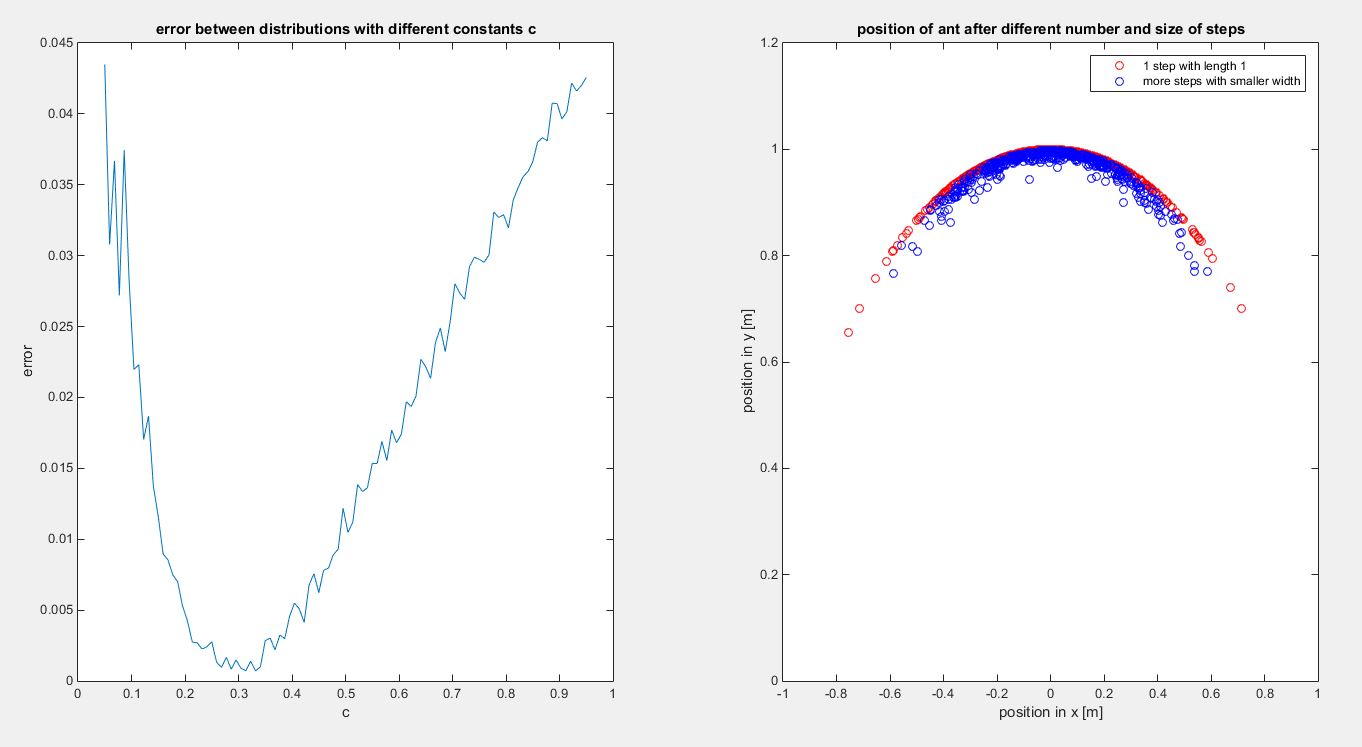
\includegraphics[scale=0.2]{./Pics/VarianceForStepWidth_plot.png} 
\caption{Variance for stepwidth}
\end{figure} 
\end{frame}




\subsection{Verification of the path integrator}
\begin{frame}
\frametitle{Verification of the path integrator}
\only<1>{ 
\begin{enumerate}
\item ant walks 12 m in a fixed direction
\item then turns an angle $\alpha$ walks 5 more meters, where it finds food
\item the ant returns with a certain error.
\end{enumerate}


\begin{figure}[H]
\centering
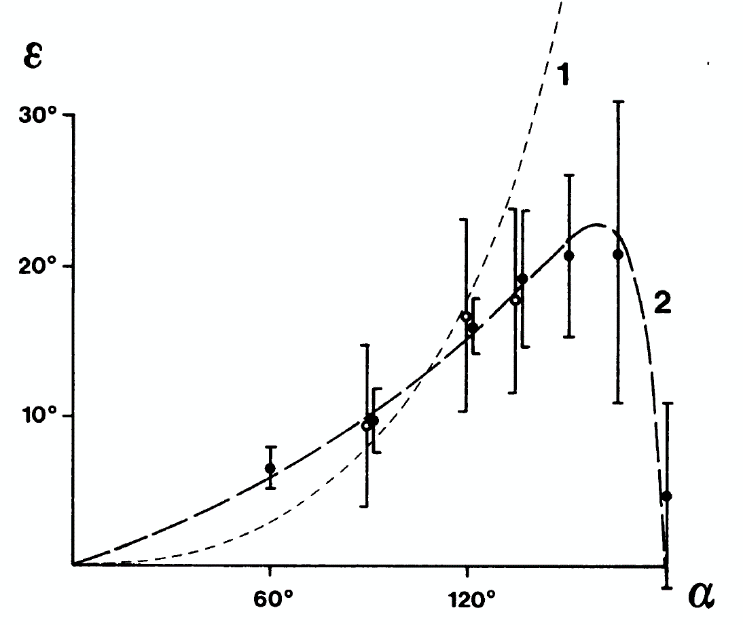
\includegraphics[scale=0.22]{./Pics/angularErrorOfWehner.png} 
\caption{Angular Error according to Wehner1988 }
\end{figure} 
}



\only<2>{ 
\begin{enumerate}
\item ant walks 12 m in a fixed direction
\item then turns an angle $\alpha$ walks 5 more meters, where it finds food
\item the ant returns with a certain error.
\end{enumerate}


\begin{figure}[H]
\centering
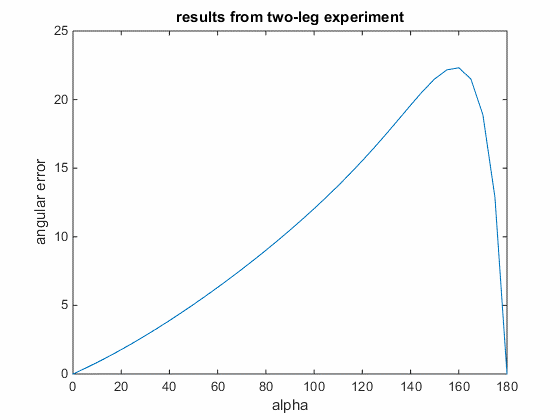
\includegraphics[scale=0.35]{./Pics/angularError.png} 
\caption{Angular error produced by our model }
\end{figure} 
}


\only<3>{ 
Comparison


\begin{figure}[H]
\centering
\includegraphics[scale=0.7]{./Pics/angularErrorCombined.png} 
\caption{Comparison }
\end{figure} 
}













\end{frame}










\end{frame}













\section{Local Orientation}
\begin{frame}
\frametitle{Local Orientation}
\begin{center}

\only<1>{
\begin{itemize}
\item familiar landmarks are memorized in the correct sequence.
\end{itemize}
}

\only<2>{
\begin{itemize}
\item familiar landmarks are memorized in the correct sequence.
\item number of steps to follow and direction representing the local vector.
\end{itemize}
}

\end{center}
\end{frame}

\section{Outlook}
\begin{frame}
\frametitle{Outlook and Conclusions}
\begin{center}

\only<1>{
\begin{itemize}
\item Does our model meet the requirements?
\item Are we able to predict ant behaviour?
\item Outlook
\end{itemize}
}










\end{center}
\end{frame}








\section{}
\begin{frame}
\frametitle{Thanks for your attention}
\begin{center}
Questions ?
\end{center}
\end{frame}


\end{document}